% !TeX spellcheck = en_US
\documentclass[11pt]{report}
\usepackage[utf8]{inputenc}
\usepackage{amsmath}
\usepackage{amsthm}
\usepackage{amssymb}
\usepackage{graphicx}
\graphicspath{ {images/} }
\usepackage{caption}
\usepackage{parskip}
\usepackage{subcaption}
\usepackage[shortlabels]{enumitem}
\usepackage{float}
\usepackage{color}   %May be necessary if you want to color links
\usepackage{hyperref}
\hypersetup{
	colorlinks=true, %set true if you want colored links
	linktoc=all,     %set to all if you want both sections and subsections linked
	linkcolor=green,  %choose some color if you want links to stand out
	bookmarksopen=true,
}
\hypersetup{linktocpage}
\usepackage[open,openlevel=1]{bookmark}

\usepackage[Lenny]{fncychap}


\usepackage[width=150mm,top=35mm,bottom=25mm,bindingoffset=6mm]{geometry}
\usepackage{fancyhdr}
\pagestyle{fancyplain}% <- use fancyplain instead fancy
\fancyhf{}
\fancyhead[R]{\thepage}
\renewcommand{\headrulewidth}{0pt}
\setlength{\headheight}{14pt}

\newtheorem{theorem}{Theorem}[section]
\newtheorem{definition}{Definition}[section]
\newtheorem{corollary}{Corollary}[theorem]
\newtheorem{lemma}[theorem]{Lemma}
\newtheorem{assumptions}[definition]{Assumptions}

\newcommand{\bbR}{\mathbb{R}}
\renewcommand\qedsymbol{$\blacksquare$}
\newcommand{\dpartial}[2]{\frac{\partial #1}{\partial #2}}
\DeclareMathOperator{\Tr}{Tr}

\setlength{\parindent}{0cm}

\usepackage{mathtools}

\NewDocumentCommand{\expect}{ e{^} s o >{\SplitArgument{1}{||}}m }{%
	\operatorname{\mathbb{E}}%     the expectation operator
	\IfValueT{#1}{{\!}^{#1}}% the measure of the expectation
	\IfBooleanTF{#2}{% *-variant
		\expectarg*{\expectvar#4}%
	}{% no *-variant
		\IfNoValueTF{#3}{% no optional argument
			\expectarg{\expectvar#4}%
		}{% optional argument
			\expectarg[#3]{\expectvar#4}%
		}%
	}%
}
\NewDocumentCommand{\expectvar}{mm}{%
	#1\IfValueT{#2}{\nonscript\;\delimsize\vert\nonscript\;#2}%
}
\DeclarePairedDelimiterX{\expectarg}[1]{[}{]}{#1}


\usepackage[sorting=none]{biblatex}
%\addbibresource{references.bib}
\addbibresource{Probabilidad.bib}
\addbibresource{PDEs ML.bib}
\addbibresource{ControlOptimizacion.bib}
\addbibresource{BSDEs.bib}

\title{Deep learning method for high dimensional PDE's}
\author{Carlos Daniel Contreras Quiroz}
\date{Day Month Year}

\begin{document}
\pagenumbering{roman} 

\begin{titlepage}
    \begin{center}
        \vspace*{1cm}
        
        \Huge
        \textbf{A deep learning method for high dimensional PDE's}
        
        \vspace{0.5cm}
        \LARGE
        An application to mean field games\\
        \vspace{0.5cm}
   
        by\\
        \vspace{0.5cm}
    
        \textbf{Carlos Daniel Contreras Quiroz}\\
        \vspace*{1cm}
        Advisor: Mauricio Junca
        
        \vfill
        
        A dissertation submitted in partial fulfillment\\
        of the requirements for the degree of\\
        Master in\\
        Mathematics\\
    
        
        \vspace{1.8cm}

        
        \Large
        at the\\Universidad de los Andes\\
        2023\\
        \vspace{1.0cm}
       
        
    \end{center}
    
\end{titlepage}



\fancyhf{} % clear all header and footer fields
\fancyhead[RO,R]{\thepage} %RO=right odd, RE=right even
\renewcommand{\headrulewidth}{0pt}

\begin{center}
    \Large
    \textbf{Deep learning methods for high dimensional PDE's}
    
    \vspace{0.4cm}
    \large
    An application to N-agent games
    
    \vspace{0.4cm}
    \textbf{Carlos Daniel Contreras Quiroz}
    
    \vspace{0.9cm}
    \textbf{Abstract}
\end{center}
Nada

\chapter*{Acknowledgements}
A mi lulú y mi pancita.Nadita.


\tableofcontents


%\listoffigures


%\listoftables


\chapter{Introduction}
\pagenumbering{arabic} 
Lorem ipsum dolor sit amet, consectetur adipisicing elit, sed do eiusmod tempor incididunt ut labore et dolore magna aliqua. Ut enim ad minim veniam, quis nostrud exercitation ullamco laboris nisi ut aliquip ex ea commodo consequat. Duis aute irure dolor in reprehenderit in voluptate velit esse cillum dolore eu fugiat nulla pariatur. Excepteur sint occaecat cupidatat non proident, sunt in culpa qui officia deserunt mollit anim id est laborum.

Lorem ipsum dolor sit amet, consectetur adipisicing elit, sed do eiusmod tempor incididunt ut labore et dolore magna aliqua. Ut enim ad minim veniam, quis nostrud exercitation ullamco laboris nisi ut aliquip ex ea commodo consequat. Duis aute irure dolor in reprehenderit in voluptate velit esse cillum dolore eu fugiat nulla pariatur. Excepteur sint occaecat cupidatat non proident, sunt in culpa qui officia deserunt mollit anim id est laborum.

Lorem ipsum dolor sit amet, consectetur adipisicing elit, sed do eiusmod tempor incididunt ut labore et dolore magna aliqua. Ut enim ad minim veniam, quis nostrud exercitation ullamco laboris nisi ut aliquip ex ea commodo consequat. Duis aute irure dolor in reprehenderit in voluptate velit esse cillum dolore eu fugiat nulla pariatur. Excepteur sint occaecat cupidatat non proident, sunt in culpa qui officia deserunt mollit anim id est laborum.

Lorem ipsum dolor sit amet, consectetur adipisicing elit, sed do eiusmod tempor incididunt ut labore et dolore magna aliqua. Ut enim ad minim veniam, quis nostrud exercitation ullamco laboris nisi ut aliquip ex ea commodo consequat. Duis aute irure dolor in reprehenderit in voluptate velit esse cillum dolore eu fugiat nulla pariatur. Excepteur sint occaecat cupidatat non proident, sunt in culpa qui officia deserunt mollit anim id est laborum.

Lorem ipsum dolor sit amet, consectetur adipisicing elit, sed do eiusmod tempor incididunt ut labore et dolore magna aliqua. Ut enim ad minim veniam, quis nostrud exercitation ullamco laboris nisi ut aliquip ex ea commodo consequat. Duis aute irure dolor in reprehenderit in voluptate velit esse cillum dolore eu fugiat nulla pariatur. Excepteur sint occaecat cupidatat non proident, sunt in culpa qui officia deserunt mollit anim id est laborum.

Lorem ipsum dolor sit amet, consectetur adipisicing elit, sed do eiusmod tempor incididunt ut labore et dolore magna aliqua. Ut enim ad minim veniam, quis nostrud exercitation ullamco laboris nisi ut aliquip ex ea commodo consequat. Duis aute irure dolor in reprehenderit in voluptate velit esse cillum dolore eu fugiat nulla pariatur. Excepteur sint occaecat cupidatat non proident, sunt in culpa qui officia deserunt mollit anim id est laborum.

\chapter{Backward stochastic differential equations and PDEs}
When we deal with deterministic optimal control problems there are two approaches one involving Bellman's dynamic programming principle and the other relying on the Pontryagin's maximum principle. The former approach leads to a partial differential equation named the Hamilton-Jacobi-Bell equation, while the latter leads to a system of ordinary differential equations which are defined backward in time. 

Suppose, that I love you. And that I hate foeul

Underlines that are blue indicate that Grammarly has detected something wrong.
The bananas are tasty
\section{Section Title}
Lorem ipsum dolor sit amet, consectetur adipisicing elit, sed do eiusmod tempor incididunt ut labore et dolore magna aliqua. Ut enim ad minim veniam, quis nostrud exercitation ullamco laboris nisi ut aliquip ex ea commodo consequat. Duis aute irure dolor in reprehenderit in voluptate velit esse cillum dolore eu fugiat nulla pariatur. Excepteur sint occaecat cupidatat non proident, sunt in culpa qui officia deserunt mollit anim id est laborum.

Lorem ipsum dolor sit amet, consectetur adipisicing elit, sed do eiusmod tempor incididunt ut labore et dolore magna aliqua. Ut enim ad minim veniam, quis nostrud exercitation ullamco laboris nisi ut aliquip ex ea commodo consequat. Duis aute irure dolor in reprehenderit in voluptate velit esse cillum dolore eu fugiat nulla pariatur. Excepteur sint occaecat cupidatat non proident, sunt in culpa qui officia deserunt mollit anim id est laborum.
Lorem ipsum dolor sit amet, consectetur adipisicing elit, sed do eiusmod tempor incididunt ut labore et dolore magna aliqua. Ut enim ad minim veniam, quis nostrud exercitation ullamco laboris nisi ut aliquip ex ea commodo consequat. Duis aute irure dolor in reprehenderit in voluptate velit esse cillum dolore eu fugiat nulla pariatur. Excepteur sint occaecat cupidatat non proident, sunt in culpa qui officia deserunt mollit anim id est laborum.

Lorem ipsum dolor sit amet, consectetur adipisicing elit, sed do eiusmod tempor incididunt ut labore et dolore magna aliqua. Ut enim ad minim veniam, quis nostrud exercitation ullamco laboris nisi ut aliquip ex ea commodo consequat. Duis aute irure dolor in reprehenderit in voluptate velit esse cillum dolore eu fugiat nulla pariatur. Excepteur sint occaecat cupidatat non proident, sunt in culpa qui officia deserunt mollit anim id est laborum.

Lorem ipsum dolor sit amet, consectetur adipisicing elit, sed do eiusmod tempor incididunt ut labore et dolore magna aliqua. Ut enim ad minim veniam, quis nostrud exercitation ullamco laboris nisi ut aliquip ex ea commodo consequat. Duis aute irure dolor in reprehenderit in voluptate velit esse cillum dolore eu fugiat nulla pariatur. Excepteur sint occaecat cupidatat non proident, sunt in culpa qui officia deserunt mollit anim id est laborum.

\section{Section Title}
Lorem ipsum dolor sit amet, consectetur adipisicing elit, sed do eiusmod tempor incididunt ut labore et dolore magna aliqua. Ut enim ad minim veniam, quis nostrud exercitation ullamco laboris nisi ut aliquip ex ea commodo consequat. Duis aute irure dolor in reprehenderit in voluptate velit esse cillum dolore eu fugiat nulla pariatur see \ref{fig:x cubed graph}. Excepteur sint occaecat cupidatat non proident, sunt in culpa qui officia deserunt mollit anim id est laborum.
\begin{figure}[ht]
\centering
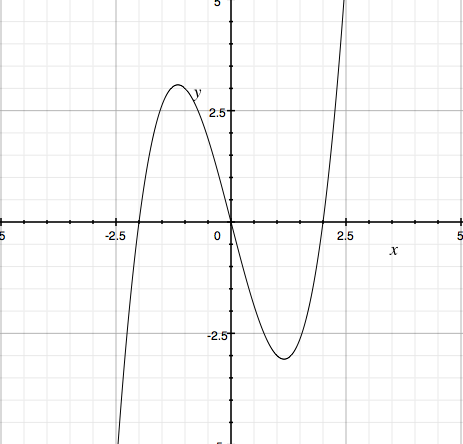
\includegraphics[scale=0.5]{graph_a}
\caption{An example graph}
\label{fig:x cubed graph}
\end{figure}

Lorem ipsum dolor sit amet, consectetur adipisicing elit, sed do eiusmod tempor incididunt ut labore et dolore magna aliqua. Ut enim ad minim veniam, quis nostrud exercitation ullamco laboris nisi ut aliquip ex ea commodo consequat. Duis aute irure dolor in reprehenderit in voluptate velit esse cillum dolore eu fugiat nulla pariatur. Excepteur sint occaecat cupidatat non proident, sunt in culpa qui officia deserunt mollit anim id est laborum.

Lorem ipsum dolor sit amet, consectetur adipisicing elit, sed do eiusmod tempor incididunt ut labore et dolore magna aliqua. Ut enim ad minim veniam, quis nostrud exercitation ullamco laboris nisi ut aliquip ex ea commodo consequat. Duis aute irure dolor in reprehenderit in voluptate velit esse cillum dolore eu fugiat nulla pariatur. Excepteur sint occaecat cupidatat non proident, sunt in culpa qui officia deserunt mollit anim id est laborum.

Lorem ipsum dolor sit amet, consectetur adipisicing elit, sed do eiusmod tempor incididunt ut labore et dolore magna aliqua. Ut enim ad minim veniam, quis nostrud exercitation ullamco laboris nisi ut aliquip ex ea commodo consequat. Duis aute irure dolor in reprehenderit in voluptate velit esse cillum dolore eu fugiat nulla pariatur. Excepteur sint occaecat cupidatat non proident, sunt in culpa qui officia deserunt mollit anim id est laborum.

Lorem ipsum dolor sit amet, consectetur adipisicing elit, sed do eiusmod tempor incididunt ut labore et dolore magna aliqua. Ut enim ad minim veniam, quis nostrud exercitation ullamco laboris nisi ut aliquip ex ea commodo consequat. Duis aute irure dolor in reprehenderit in voluptate velit esse cillum dolore eu fugiat nulla pariatur. Excepteur sint occaecat cupidatat non proident, sunt in culpa qui officia deserunt mollit anim id est laborum.

Lorem ipsum dolor sit amet, consectetur adipisicing elit, sed do eiusmod tempor incididunt ut labore et dolore magna aliqua. Ut enim ad minim veniam, quis nostrud exercitation ullamco laboris nisi ut aliquip ex ea commodo consequat. Duis aute irure dolor in reprehenderit in voluptate velit esse cillum dolore eu fugiat nulla pariatur. Excepteur sint occaecat cupidatat non proident, sunt in culpa qui officia deserunt mollit anim id est laborum.

Lorem ipsum dolor sit amet, consectetur adipisicing elit, sed do eiusmod tempor incididunt ut labore et dolore magna aliqua. Ut enim ad minim veniam, quis nostrud exercitation ullamco laboris nisi ut aliquip ex ea commodo consequat. Duis aute irure dolor in reprehenderit in voluptate velit esse cillum dolore eu fugiat nulla pariatur. Excepteur sint occaecat cupidatat non proident, sunt in culpa qui officia deserunt mollit anim id est laborum.

Lorem ipsum dolor sit amet, consectetur adipisicing elit, sed do eiusmod tempor incididunt ut labore et dolore magna aliqua. Ut enim ad minim veniam, quis nostrud exercitation ullamco laboris nisi ut aliquip ex ea commodo consequat. Duis aute irure dolor in reprehenderit in voluptate velit esse cillum dolore eu fugiat nulla pariatur. Excepteur sint occaecat cupidatat non proident, sunt in culpa qui officia deserunt mollit anim id est laborum.

Lorem ipsum dolor sit amet, consectetur adipisicing elit, sed do eiusmod tempor incididunt ut labore et dolore magna aliqua. Ut enim ad minim veniam, quis nostrud exercitation ullamco laboris nisi ut aliquip ex ea commodo consequat. Duis aute irure dolor in reprehenderit in voluptate velit esse cillum dolore eu fugiat nulla pariatur. Excepteur sint occaecat cupidatat non proident, sunt in culpa qui officia deserunt mollit anim id est laborum.

Lorem ipsum dolor sit amet, consectetur adipisicing elit, sed do eiusmod tempor incididunt ut labore et dolore magna aliqua. Ut enim ad minim veniam, quis nostrud exercitation ullamco laboris nisi ut aliquip ex ea commodo consequat. Duis aute irure dolor in reprehenderit in voluptate velit esse cillum dolore eu fugiat nulla pariatur. Excepteur sint occaecat cupidatat non proident, sunt in culpa qui officia deserunt mollit anim id est laborum.

Lorem ipsum dolor sit amet, consectetur adipisicing elit, sed do eiusmod tempor incididunt ut labore et dolore magna aliqua. Ut enim ad minim veniam, quis nostrud exercitation ullamco laboris nisi ut aliquip ex ea commodo consequat. Duis aute irure dolor in reprehenderit in voluptate velit esse cillum dolore eu fugiat nulla pariatur. Excepteur sint occaecat cupidatat non proident, sunt in culpa qui officia deserunt mollit anim id est laborum.

Lorem ipsum dolor sit amet, consectetur adipisicing elit, sed do eiusmod tempor incididunt ut labore et dolore magna aliqua. Ut enim ad minim veniam, quis nostrud exercitation ullamco laboris nisi ut aliquip ex ea commodo consequat. Duis aute irure dolor in reprehenderit in voluptate velit esse cillum dolore eu fugiat nulla pariatur. Excepteur sint occaecat cupidatat non proident, sunt in culpa qui officia deserunt mollit anim id est laborum.

Lorem ipsum dolor sit amet, consectetur adipisicing elit, sed do eiusmod tempor incididunt ut labore et dolore magna aliqua. Ut enim ad minim veniam, quis nostrud exercitation ullamco laboris nisi ut aliquip ex ea commodo consequat. Duis aute irure dolor in reprehenderit in voluptate velit esse cillum dolore eu fugiat nulla pariatur. Excepteur sint occaecat cupidatat non proident, sunt in culpa qui officia deserunt mollit anim id est laborum.

\section{Section Title}
Lorem ipsum dolor sit amet, consectetur adipisicing elit, sed do eiusmod tempor incididunt ut labore et dolore magna aliqua. Ut enim ad minim veniam, quis nostrud exercitation ullamco laboris nisi ut aliquip ex ea commodo consequat. Duis aute irure dolor in reprehenderit in voluptate velit esse cillum dolore eu fugiat nulla pariatur. Excepteur sint occaecat cupidatat non proident, sunt in culpa qui officia deserunt mollit anim id est laborum.

Lorem ipsum dolor sit amet, consectetur adipisicing elit, sed do eiusmod tempor incididunt ut labore et dolore magna aliqua. Ut enim ad minim veniam, quis nostrud exercitation ullamco laboris nisi ut aliquip ex ea commodo consequat. Duis aute irure dolor in reprehenderit in voluptate velit esse cillum dolore eu fugiat nulla pariatur. Excepteur sint occaecat cupidatat non proident, sunt in culpa qui officia deserunt mollit anim id est laborum.

Lorem ipsum dolor sit amet, consectetur adipisicing elit, sed do eiusmod tempor incididunt ut labore et dolore magna aliqua. Ut enim ad minim veniam, quis nostrud exercitation ullamco laboris nisi ut aliquip ex ea commodo consequat. Duis aute irure dolor in reprehenderit in voluptate velit esse cillum dolore eu fugiat nulla pariatur. Excepteur sint occaecat cupidatat non proident, sunt in culpa qui officia deserunt mollit anim id est laborum.

Lorem ipsum dolor sit amet, consectetur adipisicing elit, sed do eiusmod tempor incididunt ut labore et dolore magna aliqua. Ut enim ad minim veniam, quis nostrud exercitation ullamco laboris nisi ut aliquip ex ea commodo consequat. Duis aute irure dolor in reprehenderit in voluptate velit esse cillum dolore eu fugiat nulla pariatur. Excepteur sint occaecat cupidatat non proident, sunt in culpa qui officia deserunt mollit anim id est laborum.

Lorem ipsum dolor sit amet, consectetur adipisicing elit, sed do eiusmod tempor incididunt ut labore et dolore magna aliqua. Ut enim ad minim veniam, quis nostrud exercitation ullamco laboris nisi ut aliquip ex ea commodo consequat. Duis aute irure dolor in reprehenderit in voluptate velit esse cillum dolore eu fugiat nulla pariatur. Excepteur sint occaecat cupidatat non proident, sunt in culpa qui officia deserunt mollit anim id est laborum.

\subsection{SubSection Title}
Lorem ipsum dolor sit amet, consectetur adipisicing elit, sed do eiusmod tempor incididunt ut labore et dolore magna aliqua. Ut enim ad minim veniam, quis nostrud exercitation ullamco laboris nisi ut aliquip ex ea commodo consequat. Duis aute irure dolor in reprehenderit in voluptate velit esse cillum dolore eu fugiat nulla pariatur. Excepteur sint occaecat cupidatat non proident, sunt in culpa qui officia deserunt mollit anim id est laborum.

\subsection{SubSection Title}
Lorem ipsum dolor sit amet, consectetur adipisicing elit, sed do eiusmod tempor incididunt ut labore et dolore magna aliqua. Ut enim ad minim veniam, quis nostrud exercitation ullamco laboris nisi ut aliquip ex ea commodo consequat. Duis aute irure dolor in reprehenderit in voluptate velit esse cillum dolore eu fugiat nulla pariatur. Excepteur sint occaecat cupidatat non proident, sunt in culpa qui officia deserunt mollit anim id est laborum.

\chapter{Deep Learning Methods for PDEs}
Partial differential equations (PDE's) are ubiquitous among the tools for modeling complex phenomena in all sciences. However, we almost never have explicit solutions for them, making it difficult to describe those phenomenons and make accurate predictions about them. Hence, we need numerical methods to provide approximate solutions to those equations, for example, classical methods are finite differences, finite elements and spectral methods. Those rely on different discretizations of the particular problem that  we can use for calculating approximations in different forms and with varying levels of accuracy. Since the advent of fast computers and efficient tools for programming them, this process is effective for many kinds of problems.   

Now, when we attempt to solve numerically some particular problem, we need to play with the trade-off between accuracy of the approximate solution and the computational cost needed to obtain it. Indeed, with those classical methods, a small approximation error requires a finer grid, which implies more computational resources to store and process the information required by the method. In consequence, for some problems, we may not be able to calculate an accurate enough solution in a feasible computational time.

This is the case for high dimensional PDE's, for which the size of discretization usually scales exponentially with the number of points used for each dimension. For example, if we try to use a finite difference scheme in a $100$-dimensional unit square $[0,1]^{100}$ with $N$ points in each dimension, we would need $N^{100}$ points in total, making it impossible to even store them in a computer. In practice, high dimension can be considered as low as $d>4$, for which traditional methods cannot be used as regularly. This problem is known as the \textit{curse of dimensionality}, a term established by Bellman when considering problems in dynamic programming.

High dimensional PDE's appear in many contexts, such as asset pricing, image denoising, statistical physics, many-body quantum mechanics, optimal control and game theory. Therefore, there is a necessity for numerical methods that are able to overcome this difficulty. Early attempts to solve this kind of problems used the connection between stochastic diffusions and parabolic PDE's, as we seemed in the preceding chapter. In fact, if the PDE is linear, the linear Feynman-Kac \ref{thm:LinearFK} formula can be used to provide an approximate solution by computing the expectation using simulated paths of the process through the  Monte-Carlo approach. The convergence of this formulation is \hlc[Sure?]{independent} of the dimension of the underlying process, and therefore does not suffer from the curse dimensionality.

Nevertheless, if we try a similar approach using the non-linear Feynman-Kac formula \ref{thm:NonlinealFK} for more general non-linear equations, we would have to deal with solving numerically the associated BSDE. There are numerical methods to approximate the set of solution processes $(X,Y,Z)$, but they are not as simple as an Euler-Maruyama discretization for a forward process. Generally, they require the computation of conditional expectations that almost never are computationally cheap and hence is not a straightforward generalization of the former linear approach. Despite this, some progress has been made under this formulation, see for example \cite{chessari_numerical_nodate}.

Representing functions in a high dimensional space is a problem encountered in many other areas of applied mathematics. Particularly, in recent times, the analysis and inference on big amounts of data has emerged as the fascinating research area of \textit{machine learning}. Many methods have been proposed for this goal, for example, regression methods, support vector machines and tree methods. Nonetheless, the approach that has encountered more success when trying to approximate high dimensional functions using big amounts of data is deep learning.  In this setting, we parametrize functions using structures that use composition of simpler function for approximate complex ones, these structures are called neural networks. We refer the reader to \autoref{chp:ApendixNN} for a brief introduction and to \cite{higham_deep_2019} for a deeper exposition of the topic.

The idea of using this neural network parametrization of functions to solve PDE's can be tracked to the 80's, when in \cite{} a perceptron layer approximation was proposed to \hlc[Completar]{}. However, due to the high computational cost of training a neural network, a sucessfull attempt was not achieved until recently, with the works \cite{bibid}\hlc[Blablabla]{}. 

This is a very new area of research, for which many open questions remain. Particularly, it is not well understood yet if the curse of dimensionality is solved, even if there is work for certain equations that ensures it \cite{bibid}. Also, there is not yet a good understanding of why different classes of neural networks are useful to approximate certain classes of functions and how to tune adequately its parameters to do it efficiently. In consequence, even if it is possible to give a convergence proof for certain cases, most algorithms rely on empirical experimentation and heuristic arguments to provide reasonable approximate solutions.    

In this chapter we review some of these methods, implement them for toy examples and perform a comparison of speed, accuracy and practical usefulness for solving PDE's.   




\section{Free boundary problems}
\subsection{Deep BSDE method}

\subsubsection*{Merged Deep BSDE}
\subsubsection*{Residual Merged Deep BSDE}

\subsection{Raissi's method}
\subsection{Deep Splitting/Tensor train?}
\subsection{An example}
\section{Boundary problems}
\subsection{Deep Galerkin method}
\subsection{Interpolating BSDEs with PINNs}
\subsection{Reflection on Boundary}

\subsection{An example with optimal control}

\chapter{Crowd motion modeling}
We have seen how deep learning tool can be used to solve partial differential equations, even in the high dimensional setting. However, we have not solved any problem for which we do not know an exact solution or an approximate one by means of classical numerical methods. Hence, in this section we will apply the exposed methods to solve a larger problem whose solution cannot be approximated by classical numerical methods. That is the case for N-agent games, which is the main topic of this section. 
\section{N-agent games}
Classical optimal stochastic control deals with the problem of optimizing the optimal choice that a single agent should take to minimize a cost function in a random environment, see \autoref{chp:ApendixStochasticControl}.  What happens when there are many agents taking decisions to minimize their own cost that may depend on other's states and strategies? How should an agent choose its strategy to minimize its own cost knowing that other agents will try to do the same?  Such questions can be answered in the framework of stochastic differential games, for which here we give an introduction following \cite{hu_recent_nodate,han_deep_2020}.

Consider a system that consist of $N$ agents, also called players, whose states are represented by a continuous stochastic process $X^{i}_{t}\in \bbR^d$ , with $i\in \mathcal{I}:=\{1,\ldots, N\}$, that continuously take actions $\alpha_{t}^{i}$ in a control set $\mathcal{A}^i\subset \bbR^k$. The dynamics in the time interval $[0,T]$ of the controlled state process $X^i$ follows the stochastic differential equation
\begin{equation}
	\begin{split}
		&dX_t^{i}=\mu^{i}(t,\bfX_t,\bfAlp_t)dt+\sigma^{i}(t,\bfX_t,\bfAlp_t)dW_t^{i}+\sigma^{0}(t,\bfX_t,\bfAlp_t)dW_{t}^0\\
		&X_{0}^{i}=x_{0}^{i} \quad \text{ for } i\in \mathcal{I},
	\end{split}
\end{equation}
where $\mathbf{W}:=(W^0,W^1,\ldots W^N)$ are $N+1$ $m$-dimensional independent Brownian motions, $W^{i}$ are individual noises and $W^0$ is common noise for all agents, and $\bfX_t=[X_t^1,\ldots,X_t^N]$ is the joint vector for the $N$ agent dynamics with their corresponding controls $\bfAlp_t=(\alpha_t^1,\ldots,\alpha_t^N)$. The individual drift and volatility $(\mu^i,\sigma^i)$ are deterministic functions $b^{i}:[0,T]\times \bbR^{dN}\times \mathcal{A}^N\to \bbR^d\times \bbR$ and $\sigma^{i}:[0,T]\times \bbR^{dN}\times \mathcal{A}^N\to \bbR^d\times \bbR\times\bbR^{d\times m}$, which are dependent on the states and controls of every other agent.

Given a set of strategies $(\bfAlp_t)_{t\in [0,T]}$, we associate a cost/value function to player $i$ of the form
\begin{equation}
	\label{eqn:individualCost}
	v^i(t,x,\bfAlp_t):=\expect*{\int_{t}^{T}f^i(t,\bfX_t,\bfAlp_t)dt +g^i(\bfX_T)\Big| X_t^i=x},
\end{equation}
where the running cost $f^i:[0,T]\times \bbR^{dN}\times \mathcal{A}^N\to \bbR$ and the terminal cost $g^i:\bbR^{dN}\to \bbR$ are deterministic measurable functions.

Each player will try to minimize its respective total cost
\begin{equation}
	\label{eqn:total_cost}
	J^i_0(\bfAlp_t):=v(0,x^i_0,\bfAlp_t),
\end{equation}  choosing adequately $(\alpha^{i}_t)_{t\in[0,T]}$ within the set of admissible strategies $\mathbb{A}^i$. The choice of this set describes measurability and integrability of $\alpha_t^i$. For example, if we choose $\mathbb{A}^i=\mathbb{A}=\mathbb{H}^2_T(\mathcal{A})$, the space of square integrable $\bm{W}$-progressively measurable $\mathcal{A}$-valued processes, the $\alpha$ is said to be a \textit{open loop control}, because it only uses the information of the noise that has occurred. If instead we choose $\mathbb{A}^i$ as the set $\mathbb{H}_{\bfX}^2(\mathcal{A})$, the set of square integrable  $\bfX$-measurable processes, the $\alpha_t$ is a \textit{closed loop markovian control}\hlc[Revisar definicion del espacio, ¿Cuando es no medible?]{}, as it uses information of the current state $\bfX_t$.

In a noncooperative game, there is an important notion of optimality termed \textit{Nash equilibrium}, which refers to a set of strategies for all agents such that no one has an incentive to deviate in order to reduce its own cost. Explicitly, we have the following definition
\begin{definition}
A tuple $\bfAlp^*=(\alpha^{1,*},\ldots,\alpha^{N,*})\in \mathcal{A}^1\times \cdots \times \mathcal{A}^N$ is said to be a Nash equilibrium if for all $i\in\mathcal{I}$ and any $\beta^i\in\mathcal{A}^i$ we have that
 $$J^{i}(\bfAlp)\leq J^i(\alpha^{1,*},\ldots,\alpha^{i-1,*},\beta^i,\alpha^{i+1,*},\ldots ,\alpha^{N,*})$$,
 where on the rigth-hand side the strategy $(\alpha^{1,*},\ldots,\alpha^{i-1,*},\beta^i,\alpha^{i+1,*},\ldots ,\alpha^{N,*})$ is used to solve for $\bfX$ in the dynamics equation \eqref{eqn:individualCost}. Particularly, if we search for a \textit{markovian Nash equilibrium}, we require the functions $\alpha^i_t$ to be of the form $\alpha^i_t=\alpha^i(t,\bfX_t)$, for $\alpha^i$ a measurable function.  
\end{definition}

\hlc[Aclarar existencia de equilibrios? Convixidad del hamiltoniano en state and control variables]{}. Finding such equilibria is an important, yet difficult task to acomplish. In the markovian setting, the equilibrium is related to solving N coupled Hamilton-Jacobi-Bellman equations. Consider the dynamics for the joint vector 
\begin{equation}
	\label{eqn:X_dynamics}
	\begin{split}
&d\bfX_t=\mu(t,\bfX_t,\bfAlp(t,\bfX))dt+\Sigma(t,\bfX_t,\bfAlp(t,X_t))d\bm{W}_t\\
&\bfX_0=\bm{x}_0,
	\end{split}
\end{equation}
where we used the vector notation stated before and the joint noise matrix and drift given by
\begin{equation}
	\mu=\begin{bmatrix}
		\mu^1 \\
		\mu^2 \\
		\vdots   \\
		\mu^N
	\end{bmatrix}
	\quad\quad\quad
	\Sigma=\begin{bmatrix}
		\sigma^0 & \sigma^1\\
		\sigma^0 & \sigma^2\\
		\vdots   &  \vdots\\
		\sigma^0 & \sigma^N
	\end{bmatrix}.
\end{equation}

Then, the optimal value function for agent $i$ satisfies the Hamilton-Jacobi-Bellman equation given by
\begin{equation}
	\begin{split}
	&\dpartial{u^i}{t}+H^i(t,\bm{x},\bfAlp,D_x v^i,D_{xx} v^i)=0\\
	&v^i(T,x)=g^i(x),
	\end{split}
\end{equation}
where $H^i$ is the Hamiltonian function 
\begin{equation}
	\label{eqn:Hamiltonian}
	\begin{split}
		H^i(t,\bm{x},\bfAlp,p,q)&=\inf_{\alpha^i\in \mathcal{A}^i}\{\mu(t,\bm{x},\bfAlp)\cdot p+f^i(t,\bm{x},\bfAlp)+\frac{1}{2}\Tr(\Sigma\Sigma'(t,\bm{x},\bfAlp) q)\}\\
		&:=\inf_{\alpha^i\in \mathcal{A}^i}\{G^i(t,\bm{x},\bfAlp,p,q)\}.
	\end{split}
\end{equation}

The minimization over $\alpha^i$ should be carried while taking $(\alpha^1,\ldots,\alpha^{i-1},\alpha^{i+1},\ldots,\alpha^N)$ given and fixed. Note that this system of equations for $i\in\mathcal{I}$ is implicitly coupled through the joint control $\bfAlp$ because it depends directly on every $v^i$ from which we derive each $\alpha^i$.

\section{Deep Fictitious Play}
If we were able to solve the latter coupled system of partial differential equations, we would be able to find the strategy that each player must follow to minimize its cost if every other player behaves as expected.  However, this is not an achievable due to the complexity of the system.

Hence, the idea of \textit{fictitious play} was introduced by Brown \cite{brown_notes_1949} to decouple this N-player game into N individual decision problems where opponents' strategies are fixed and assumed to follow their past play. If we solve these problems iteratively using the opponents' strategy  at $(m-1)'s$ stage to compute the optimal strategy at stage $m$, we may find the Nash equilibrium of the system, if it exists. In \cite{han_deep_2020}, each of the individual decision problems is solved using the HJB equation and the deep learning methods we have studied.  

To describe this process mathematically, let's denote by $\mathcal{A}^i\subset \bbR^k $ the range player $i$'s strategy $\alpha^i$, and $\mathcal{A}:=\bigotimes_{i=1}^{N}\mathcal{A}^i$ the control space for all agents. Also, denote $\mathcal{A}^{-i}:=\bigotimes_{j\neq i}\mathcal{A}^j$ the control space for all agents by $i$. A similar notation applies for $\mathbb{A}^i$,$\mathbb{A},\mathbb{A}^{-1}$, the sets of measurable functions in which we search for controls.

Likewise, denote $\bfAlp^{-1}=(\alpha^1,\ldots,\alpha^{i-1},\alpha^{i+1},\ldots,\alpha^{N})$ the set of all agents' strategies excluding player $i$'s. A superscript $m$ in $\bfAlp^m$ denotes the set of strategies of all players at stage $m$. When both superscripts are present, $\bfAlp^{-i,m}$ it denotes the set of strategies of all players but $i$'s at stage $m$. Finally, we use the notation $(\alpha^i,\bfAlp^{-i,m})=:(\alpha^{1,m},\ldots,\alpha^{i-1,m},\alpha^i,\alpha^{i+1,m},\ldots,\alpha^{N,m})$

To start the iterations, assume we have an initial guess set of strategies $\bfAlp^0$. At stage $m+1$, all players observe $\bfAlp^m$, and the decision problem for player $i$ is 
\begin{equation}
	\inf_{\alpha^i \in \mathbb{A}^i} J_0^i((\alpha^i,\bfAlp^{-i,m}))
\end{equation},
where $J_0^i$ is defined in  equation \eqref{eqn:total_cost} and $\bfX_t$ satisfies \eqref{eqn:X_dynamics} with $\bfAlp$ being replaced by $(\alpha^i,\bfAlp^{-i,m})$. The optimal strategy for player $i$, if it exists, is denoted by $\alpha^{i,m+1}$. The set of all optimal strategies for $i\in\mathcal{I}$ together form $\bfAlp^{m+1}$.

Due to the markovianity associated to these problems, each can be translated in a Hamilton-Jacobi-Bellman equation for the value function $V^{i,m+1}(t,\bm{x})$ of the form
\begin{equation}
	\label{eqn:HJB_m_stage}
	\begin{split}
		&\dpartial{V^{i,m+1}}{t}+H^{i}(t,\bm{x},(\alpha^i,\bfAlp^{-i,m}),D_x V^{i,m+1},D_{xx} V^{i,m+1})=0\\
		&V^{i}(T,\bm{x})=g^i(\bm{x}),
	\end{split}
\end{equation}
where $H^{i}$ is defined in \eqref{eqn:Hamiltonian}. 

If this equation has a solution, the optimal strategy for player $i$ at stage $m+1$ is given by the minimizer of the Hamiltonian function
\begin{equation}
	\alpha^{i,m+1}=\argmin_{\alpha^i\in\mathcal{A}^i} G^i(t,\bm{x},(\alpha^i,\bfAlp^{-i,m}),D_x V^{i,m+1},D_{xx} V^{i,m+1}).
\end{equation}

Solving these $N$ uncoupled equations completes one stage in the fictitious play. If we solve them using deep learning methods, we call this algorithm \textit{deep fictitious play}, see \cite{han_deep_2020,hu_recent_nodate}. 

As today, we have not found general necessary conditions for this algorithm to converge to a Nash equilibrium. Indeed, we may face many problems, for example, equation \eqref{eqn:HJB_m_stage} may not have a solution for some not regular enough $\bfAlp^0$. Even more there is nothing that guarantees that $\bfAlp^m$ will converge, much less that it does so to a Nash equilibrium. In fact, there are numerous examples where it converges and where it does not, and there is not a clear pattern to evidence when it should work.
\section{An example}
Nevertheless, we will not worry too much about convergences issues and will test it numerically using the PDE solvers we have studied. 
Consider again the unbounded LQR problem in \autoref{subsec:example_LQR}. Suppose now that we can't control all players at the same time while trying to minimize a global cost function, i.e, there is not a central planner. However, every particle is able to choose its own control that minimizes it's own cost function. As before, the $i$-th particle state $X^i\in \bbR^2$ is described by the dynamics
\begin{equation}
	\begin{split}
	&dX_t^i=2\sqrt{\lambda} \alpha^i_t dt +\sqrt{2\nu} dW^i_t\\
	&X_0^i=x_0^i,
	\end{split}
\end{equation} 
where $\alpha^i_t$ is the respective $i$-th particle control function taking values in $\bbR^2$. The joint state vector is $\bfX=(X^1,\ldots,X^N)$ and the joint control is $\bfAlp=(\alpha^1,\ldots,\alpha^N)$.

Each particle is trying to minimize individually the cost 
\begin{equation}
	J^i(\alpha^i_t)=\mathbb{E}\left[\int_{0}^{T}(|\alpha^i_t|^2+F^i(t,\bfX_t)) dt +g^i(\bfX_T)\right],
\end{equation}   
irrespective of what every other particle does. Here we denoted by 
\begin{equation}
	F^i(t,\bfX_t)=C\sum_{j \neq i} e^{-\frac{|X^i-X^j|^2}{\sigma}}
\end{equation}
and 
\begin{equation}
	g^i(\bfX_T)=|X_i|^2.
\end{equation}

Hence, if we try to apply the deep fictitious play algorithm to find a Nash equilibrium for this problem, at stage $m+1$ we would need to solve all the Hamilton-Jacobi-Bellman equation for the player $i$'s value function $V^{i,m+1}$ given all other's player strategies $\bfAlp^{-i,m}$
\begin{equation}
	\label{eqn:HBJ_nomin}
	\dpartial{V^{i,m+1}}{t}+\inf_{\alpha^i}\left\{2\sqrt{\lambda}(\alpha^i,\bfAlp^{-i,m})\cdot \nabla V^{i,m+1} +|\alpha^i|^2+F^i(t,\bfX_t)+\nu \Delta V^{i,m+1}\right\}=0,
\end{equation}
subject to the terminal condition
\begin{equation}
	V^{i,m+1}(T,\bfX)=g^i(\bfX_T).
\end{equation}
The infimum of this equation can be obtained analytically, being achieved at $\alpha^i=-\sqrt{\lambda}\nabla_i V$, where $\nabla_i$ denotes the operator $\nabla_i V=(\partial_{x^i}V,\partial_{y_i}V)$. Then, inserting this infimum in \eqref{eqn:HBJ_nomin} we obtain
\begin{equation}
	\dpartial{V^{i,m+1}}{t}-\lambda|\nabla_i V^{i,m+1}|^2+2\sqrt{\lambda}\bfAlp^{-i,m}\cdot \nabla_{-i} V^{i,m+1}+F(t,\bfX)+\nu\Delta V^{i,m+1}=0,
\end{equation}
where we use the notation $\nabla_{-i} V= (\partial_{x_1}V,\partial_{y_1}V,\ldots,\partial_{x_{i-1}}V,\partial_{y_{i-1}}V,\partial_{x_{i+1}}V,\partial_{y_{i+1}}V,\ldots,\partial_{x_N}V,\partial_{y_N}V)$.

Now, to use the deep learning solvers we have seen, we recast this equation in the form \eqref{eqn:FKNolinealCh2} by choosing 
\begin{equation}
	\mu^i(t,\bfX)=2\sqrt{\lambda}\begin{bmatrix}
		\alpha^1(t,\bfX) \\
		\vdots\\
		\alpha^{i-1}(t,\bfX) \\
		0\\
		\alpha^{i+1}(t,\bfX)\\
		\vdots   \\
		\alpha^N(t,\bfX)
	\end{bmatrix}
	\quad\quad\quad
	\sigma^i(t,\bfX)=\sqrt{2\nu}\mathbb{I}_{2N\times 2N}
\end{equation}
and
\begin{equation}
	f^i(t,\bfX,V(t,\bfX),\nabla V(t,\bfX))=-\lambda|\nabla_i V|^2+F^i(t,\bfX),
\end{equation}
where we dropped the $m$ superscripts for simplicity.

Note that, in the case we solved before, all $f^i$ and $g^i$ are symmetric when interchanging players' names. Therefore, in each stage of the algorithm we need to calculate only one control that would work for every other player in the next stage of the algorithm.  

We apply this method to solve the above mentioned problem. We do not found a good form to measure accuracy of solutions in each stage of the algorithm, then, the only empirical evidence we have that the iterations converged is that the simulated trajectories were similar to those in the centralized problem. 

We ran the simulation using the same parameters as in the centralized case, and effectuated 30 iterations of the deep fictitious play. A plot of a trajectory path obtained using the optimized controls is shown in \autoref{fig:OptimalDeepFic}. Note that it resembles the optimal centralized path we found earlier, however, we do not have a systematic way to perform comparison of both solutions, as we have not carried an error analysis involved in solving the equation in each stage.

\begin{figure}[H]
	\centering
	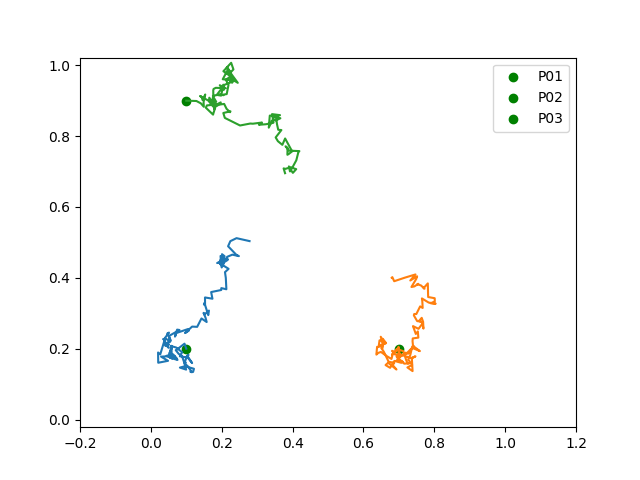
\includegraphics[width=0.7\linewidth]{images/OptimalLQRDeepFictitus.png}
	\caption{Optimal path for exiting the room}
	\label{fig:OptimalDeepFic}
\end{figure}



\chapter{An application}
Hola

\chapter{Conclusion}
In this work we evidenced the usefulness of various deep learning methods to solve partial differential equations. We applied the to solve optimal control problems using the Hamilton-Jacobi-Bellman equation in dimension 6, which is not accessible through traditional discretization methods. We implemented them in the Python programming language using the Pytorch library for automatic differentiation and neural networks tools.

These methods are very prone to error, as there are many hyperparameters that we need to tune to achieve optimal convergence. When we select them wrong, the process could even diverge. There is not a general formula to make them work in every case.

There is further work we did not accomplish due to time limitations. Our original objective was to solve an N-player game with a bigger N $(N>100)$ to compare with solutions provided by the mean field approach, see for example\cite{achdou_mean_2020}. However, boundary conditions supposed a hard problem we have not solved yet, but we expect to figure out in a near future. Also, we may solve big centralized optimal control problems to compare them with the equivalent in the limit McKean-Vlasov control problem, see \cite{carmona_control_2013}. We may be able to study the degeneration of optimal state when there is not a centralized control, and instead every player is trying to optimize its own function.

We have many ideas to be implemented. Here we list some of them 
\begin{enumerate}
	\item To take into account boundary conditions while being able to access accurately derivatives of the solution to calculate controls, we plan to try reflecting and stopping the process upon contact with a certain part of the boundary, adjusting the Deep BSDE method to include these new conditions. Preliminary results suggest that it may work, but further analysis should be done to justify this procedure theoretically.
	\item The DGM was not useful to solve bigger control problems with interaction between the particles. Our hypothesis is that this difficulty is due to the sampling step of interior points that not captures sufficient information for the solution to be accurate. Our idea is to device a method to sample points in important regions of the $N$-dimensional domain, where the solution is not well approximated by uniform sampling.
	\item In a similar spirit, maybe using a different way to produce sample paths driving them to certain regions of the domain that may be problematical would benefit convergence speed, see for example \cite{nusken_solving_2023}. 
\end{enumerate}    

\appendix
\chapter{Neural Networks}
Appendix goes here...


\printbibliography
\end{document}
